%===========[ PREAMBLE ]========================================================
\documentclass[11pt]{article}
\usepackage[utf8]{inputenc}
\usepackage[english]{babel}
\usepackage[a4paper, top=0.98in, bottom=0.79in, left=0.98in, right=0.98in]{geometry}
\usepackage{graphicx}
\usepackage{tabularx}
\usepackage{fancyhdr}
\usepackage{setspace}
\usepackage{titlesec}
\usepackage{enumitem}
\usepackage{todonotes}
\usepackage{csquotes}
\usepackage{listings}
\lstset{language=SPARQL,breaklines=true}
\usepackage{siunitx}
\usepackage[labelsep=period]{caption}
\usepackage{mwe}
\usepackage{xfrac}
\usepackage[colorlinks=true,urlcolor=blue]{hyperref}
\usepackage{cleveref}
\usepackage{aurl}
\daurl{bb}{http://www.snik.eu/ontology/bb/}
\daurl{ob}{http://www.snik.eu/ontology/bb/}
\daurl{meta}{http://www.snik.eu/ontology/meta/}
\graphicspath{{./img/}}
%\usepackage[backend=biber, style=ieee]{biblatex} %For bibliography management with biblatex
%\addbibresource{/path/to/bib/file/example.bib} %Change path to your own .bib file


% ==========[ FONT ]============================================================
%For the font of the document uncoment one of the following options.
%If using pdflatex compiler the follwoing commands will provide an arial-like
%font (helvetica)
\usepackage{helvet}
\renewcommand{\familydefault}{\sfdefault}
%If using xelatex compiler the follwoing commands will provide arial font
%\usepackage{fontspec}
%\setmainfont{Arial}

%===========[ FORMAT ]==========================================================
%Please do not edit or remove these lines
\pagenumbering{gobble}
\setlength{\parskip}{6pt}
\setlist[1]{topsep=0pt,itemsep=-5pt}
\addto\captionsenglish{\renewcommand{\figurename}{Figure}}
\addto\captionsenglish{\renewcommand{\tablename}{Table}}
\titlespacing*{\section}{0pt}{10pt}{4pt}
\titlespacing*{\subsection}{0pt}{0ex}{0pt}
\titlespacing*{\subsubsection}{0pt}{0pt}{0pt}
\titlespacing*{\paragraph}{0pt}{6pt}{6pt}
\captionsetup{belowskip=0pt,skip=6pt,labelfont=bf}%justification=raggedright,singlelinecheck=false
\makeatletter
\renewcommand{\maketitle}{
    \begin{flushleft}
        \footnotesize{Placeholder Name of the conference}\\\medskip
        \footnotesize{Placeholder Session title}\\\medskip
        \footnotesize{https://doi.or/10........ DOI placeholder (WILL BE FILLED IN BY TIB Open Publishing)}\\\medskip
        \footnotesize{\textcopyright\ Authors. This work is licensed under a \href{https://creativecommons.org/licenses/by/4.0/}{Creative Commons Attribution 4.0 International License}}\\\medskip
        \footnotesize{Published: (WILL BE FILLED IN BY TIB Open Publishing)}\\
    \end{flushleft}
    \begin{center}
        \LARGE\textbf{\contribtitle}\\\smallskip
        \Large{\contribsubtitle}
    \end{center}
    \normalsize{\firstauthor, \secondauthor, and \thirdauthor}
    \begin{center}
        \textsuperscript{1}\footnotesize{\firstauthoruniv}\\\medskip
        \textsuperscript{2}\footnotesize{\secondauthoruniv}\\\medskip
        \textsuperscript{3}\footnotesize{\thirdauthoruniv}\\\medskip
    \end{center}}
\makeatother

%===========[ TITLES ]==========================================================
%Chnage to your own information
%\newcommand{\contribtitle}{FAIR Knowledge Graphs for the Management of Health Information Systems}
\newcommand{\contribtitle}{SNIK Graph}
\newcommand{\contribsubtitle}{Visualizing Knowledge about Management of Hospital Information Systems}
%\newcommand{\contribsubtitle}{Graph-Based Exploration of an Hospital Information Systems}
\newcommand{\firstauthor}{Konrad Höffner\textsuperscript{1[https://orcid.org/0000-0001-7358-3217]}}
\newcommand{\firstauthoruniv}{Institute for Medical Informatics, Statistics and Epidemiology (IMISE), Germany}
\newcommand{\secondauthor}{Thomas Pause\textsuperscript{2[https://orcid.org/1111-2222-3333-4444]}\todo{Thomas: deine orcid ggnf. erstellen und hier eintragen }}
\newcommand{\secondauthoruniv}{Institute for Medical Informatics, Statistics and Epidemiology (IMISE), Germany}
\newcommand{\thirdauthor}{Franziska Jahn\textsuperscript{3[https://orcid.org/0000-0002-7687-8544]}}%\todo{fj: orcid bitte anpassen}
\newcommand{\thirdauthoruniv}{Institute for Medical Informatics, Statistics and Epidemiology (IMISE), Germany}

%===========[ CONTENT ]=========================================================
\begin{document}
\maketitle

\paragraph{Abstract.}% The abstract should summarize the contents of the paper in short terms, i.e. in up to 250 words.
Students of medical informatics need to internalize complex relations between large amounts of concepts of health information systems (HIS) and their management.
We present SNIK Graph, a graph-based linked data visualization web application that supports teaching textbook knowledge about HIS management.
\paragraph{Keywords:} Linked open data, health information systems, information management

\section*{Introduction}%
[FJ:] Medical and health informatics integrates knowledge of business information systems, computer science and medicine. As a comparatively young research discipline, it lacks of a uniform terminology, especially for describing health information systems and their management. However, preparing students for practical or scientific work in the domain of health information systems requires an integrated system of concepts linking the terms of the different disciplines. SNIK, the semantic network of information management in hospitals, is an ontology linking the knowledge of the textbooks (Winter et al. 2011, Ammenwerth et al. 2014, Heinrich et al. 201x \todo{ QUELLEN einfügen}), the IT4IT standard \todo{ QUELLE einfügen}, and knowledge about information management at a certain German university hospital. It thus integrates theoretical knowledge of medical informatics and information systems as well as practical knowledge from industry and a health institution. The SNIK ontology is represented by SNIK Graph. [FJ] \todo{Konrad: Mir hatte hier am Anfang ein einführender Text gefehlt. Schau mal, ob das so passt.}

SNIK Graph is a web application\footnote{\url{http://www.snik.eu/graph}} that visualizes RDF resources as nodes and triples as edges of a graph.
The graph is visualized using the Cytoscape.js~\cite{cytoscapejs} library with the force-directed Euler layout. %, see%~\cref{fig:snik-graph-overview}.
With several thousand classes, specific parts of SNIK can be hard to discern.
Thus, there are several options to view subgraphs of SNIK, for example to show only a specific chapter of a book to prepare a lecture about a specific topic.
Users can also search for and restrict the view to a single class and then show the neighbourhood of that class %(see \cref{fig:snik-graph-circle-star})
 and subsequently the neighbourhood of selected neighbours of the previous step.
SNIK Graph can also calculate the shortest path to between classes.
Path and neighourhood operations are joined in the \enquote{spider worm}
%(see \cref{fig:snik-graph-spiderworm})
, which consists of the shortest path between a start node and an end node together with the end node’s neighbourhood, illustrate the context of a concept.


\subsection*{Motivation}%
Students of medical informatics need to\todo{Vorschlag von Michelle: Dozenten können Ausschnitte des Graphen verwenden um in Vorlesungen den Zusammenhang von Konzepten vereinfacht darzustellen bzw. die Studenten diese Zusammenhänge durch Recherche im Graphen erarbeiten lassen. } internalize complex relations between large amounts of concepts of health information systems and their management~\cite{visualizationoflargeontologies}.
Graph-based Linked Data visualization~\cite{linkeddatavisualization} is well suited for this task but the available tools do not fit our requirements~\cite{visualizationoflargeontologies}.
%\cite{snikgraphposter}

%A large amount of relevant knowledge is freely available as Linked Open Data.
%This structured approach is well suited for consumption by machines but basic access mechanisms like the text-based RDF serializations and SPARQL queries are not well suited for humans for large knowledge bases, especially for non-expert users.
%While the Semantic Web field has been providing a wealth of knowledge and is increasingly adopted by mainstream industries, not all use cases are yet supported by easy-to-use tools~\cite{semanticwebfield}.
%One such use case is graph-based exploration, where RDF data is displayed as a directed graph, with the resources as nodes and the triples as edges.
%As existing approaches \iffalse(see \cref{sec:relatedwork})\fi do not satisfy the needs of the students and researchers for exploring Hospital Information Management as Linked Open Data in the SNIK ontology~\cite{sniktec}, we implement \emph{SNIK Graph} as an easy-to-use graph-based web application, which we present in the following.
%To minimize duplicated 
%One such area is exploration, where users intuitively 
%Easy-to-use and freely available tools exist for 
%However, there is a lack of easy-to-use tools along the whole lifecycle of data~\cite{semanticwebfield}.
% - software is hard to publish
%The SNIK ontology~\cite{sniktec} contains knowledge about the management of hospital information systems.
%The SNIK ontology models a typical hospital information system as a complex structure of roles (who), functions (does what) and entity types (information needed).

\cite{ontologybased}
\cite{sniktec}

\subsection*{Design Goals}
SNIK Graph's original main goal is to present knowledge extracted from text books to users that may not have any Semantic Web experience.
The time and cognitive load of the users required to install and operate the application should be as low as possible, so that they can focus on the data at hand and experience a benefit compared to only reading the textbook, such as when studying for an exam.
As such, SNIK Graph is designed as a a web application, so that it is operating system agnostic and does not need to be installed. 

When showing instances, each RDF triple maps to an edge between two nodes representing its subject and object.
When visualizing ontologies, edges between class nodes need to represent domain-range pairs and OWL restrictions.

Users should see the structure of the whole graph at once, but also be able to start at a certain resource and explore its neighbourhood incrementally.
\todo{Vorschlag von Michelle: Verwendung in der Lehre setzt intuitive/leicht erlernbare Benutzung des Graphen voraus um zu vermeiden wertvolle Vorlesungszeit an ein Tutorial zu verlieren --> Bekannet Tastaturshortcuts, Drag and Drop, übersichtliches }

\section*{Implementation}
Following the design goals, SNIK Graph is implemented in JavaScript using the graph visualization library Cytoscape.js~\cite{cytoscape}.
SNIK Graph is freely available as open source software at \footnote{\url{https://github.com/imise/snik-cytoscape.js}}.
SNIK is loaded from the given SPARQL endpoint using fetch commands.

% version 3.18.0
\label{sec:relatedwork}
\section*{Related Work}
\todo{thomas, please finish this section, does not need to be long. Or remove the section and only cite the book? or include it in the respective parts?}
Different techniques of Linked Data visualization are motivated and described in \cite{linkeddatavisualization}, including graph-based visualization.

%In the course of the SNIK project

% booktabs not allowed for this conference AFAIK
\iffalse
\begin{table}[h!]
    \centering
    \caption{Alternative Graph-based visualization tools.}
	\label{tab:relatedwork}
    \begin{tabularx}{\linewidth}{|X|X|X|X|X|X|}
        \hline
        \textbf{Tool}			& \textbf{Free} & \textbf{Plattform}	&\textbf{demo link}	&\textbf{Ontology}	&\textbf{Scales} \\ \hline
        IsaViz					& ?				& Java					& ?			&?					&?\\ \hline
        OSMoSys					& ?				& Web					& dead			&?					&?\\ \hline
        LODeX					& ?				& Web					& dead			&?					&?\\ \hline
    \end{tabularx}
\end{table}
\fi

\todo{kh: i think osmosys is not so relevant}
\emph{OSMoSys} is an experimental prototype of a web application using the Sigma.js graph drawing library.
It and handles large graphs using a level-of-detail system.
However, the demo is not accessible anymore and the code is not freely available.
Thus the maximum graph size and performance cannot be determined.

% tarsier: 3d visualization in planes. could be used for entity type vs role vs function. open source but build error.

\emph{}
% if no answer: However, there is no .
% demo link given in paper at http://www.hyperbody.nl/demo/osmosys only shows a video, author is asked for demo, repo, free and open source via email by KH
% based on sigma.js

\section*{Meta Model}
\begin{figure}[h!]
    \centering
    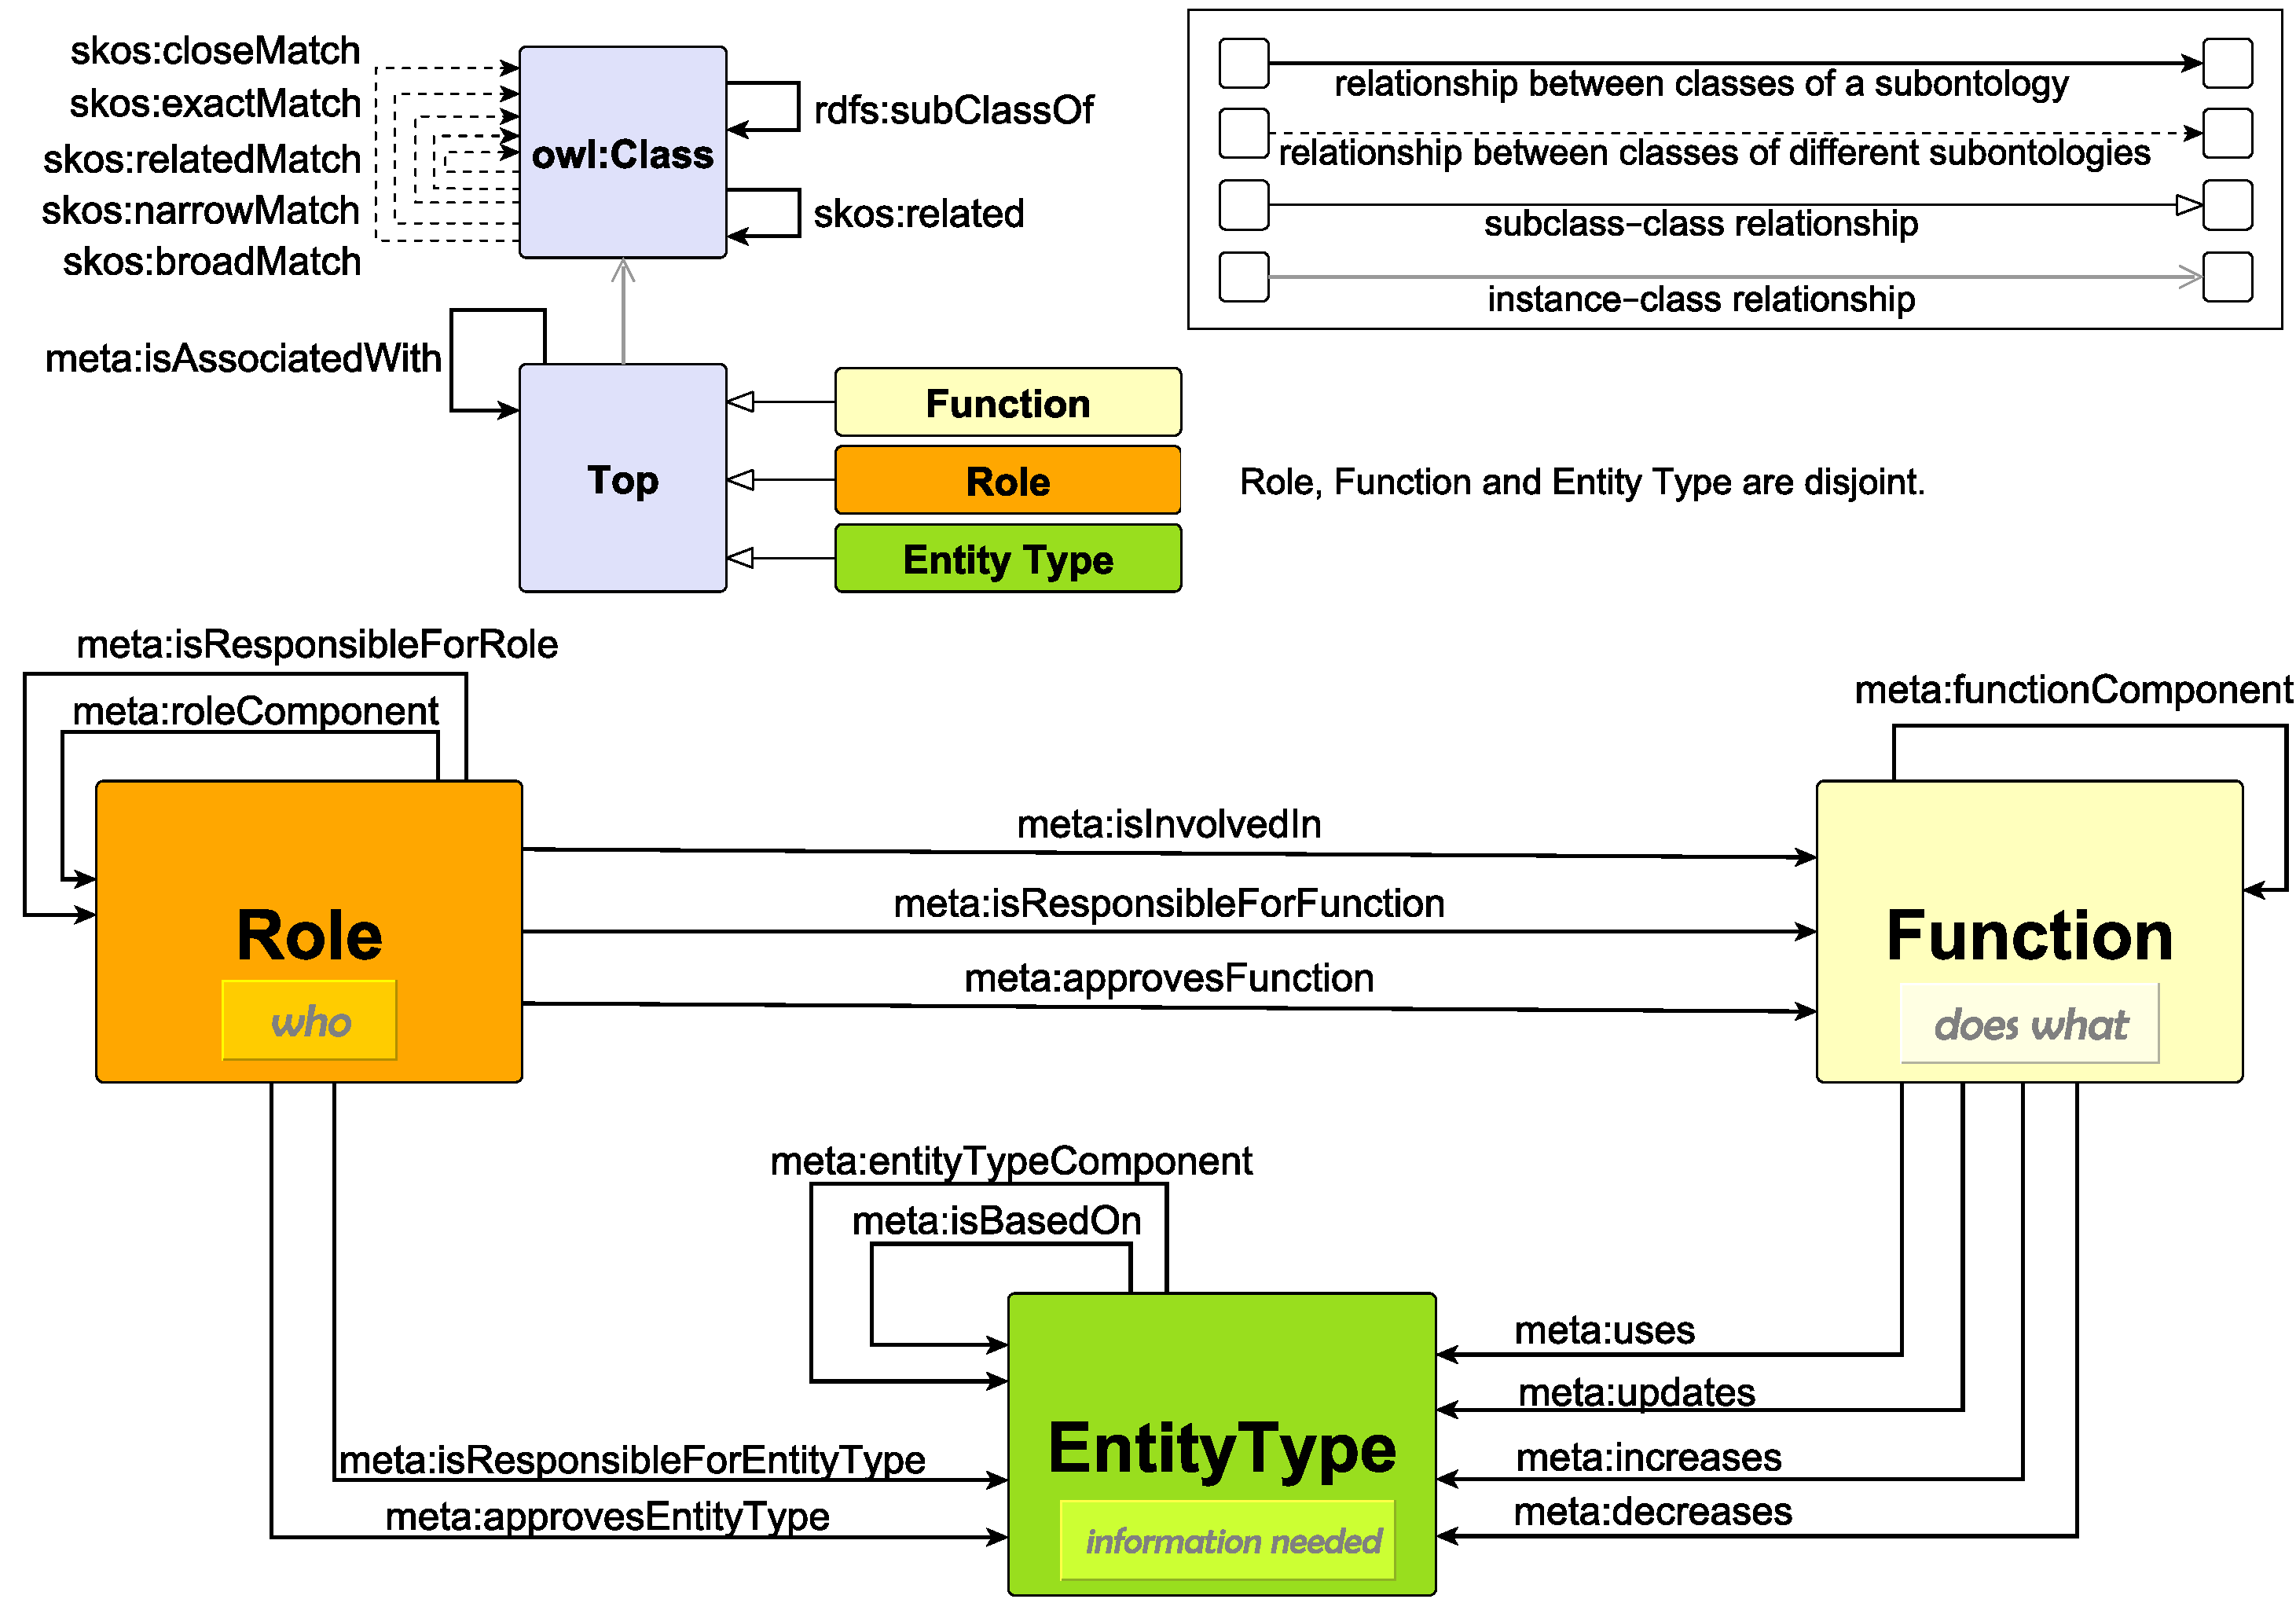
\includegraphics[width=\linewidth]{metamodel9s.pdf}
    \caption{The Meta Model of the SNIK Ontology.}\label{fig:metamodel}
\end{figure}


\section*{Features}
\subsection*{Compound Layout}
\begin{figure}[h!]
    \centering
    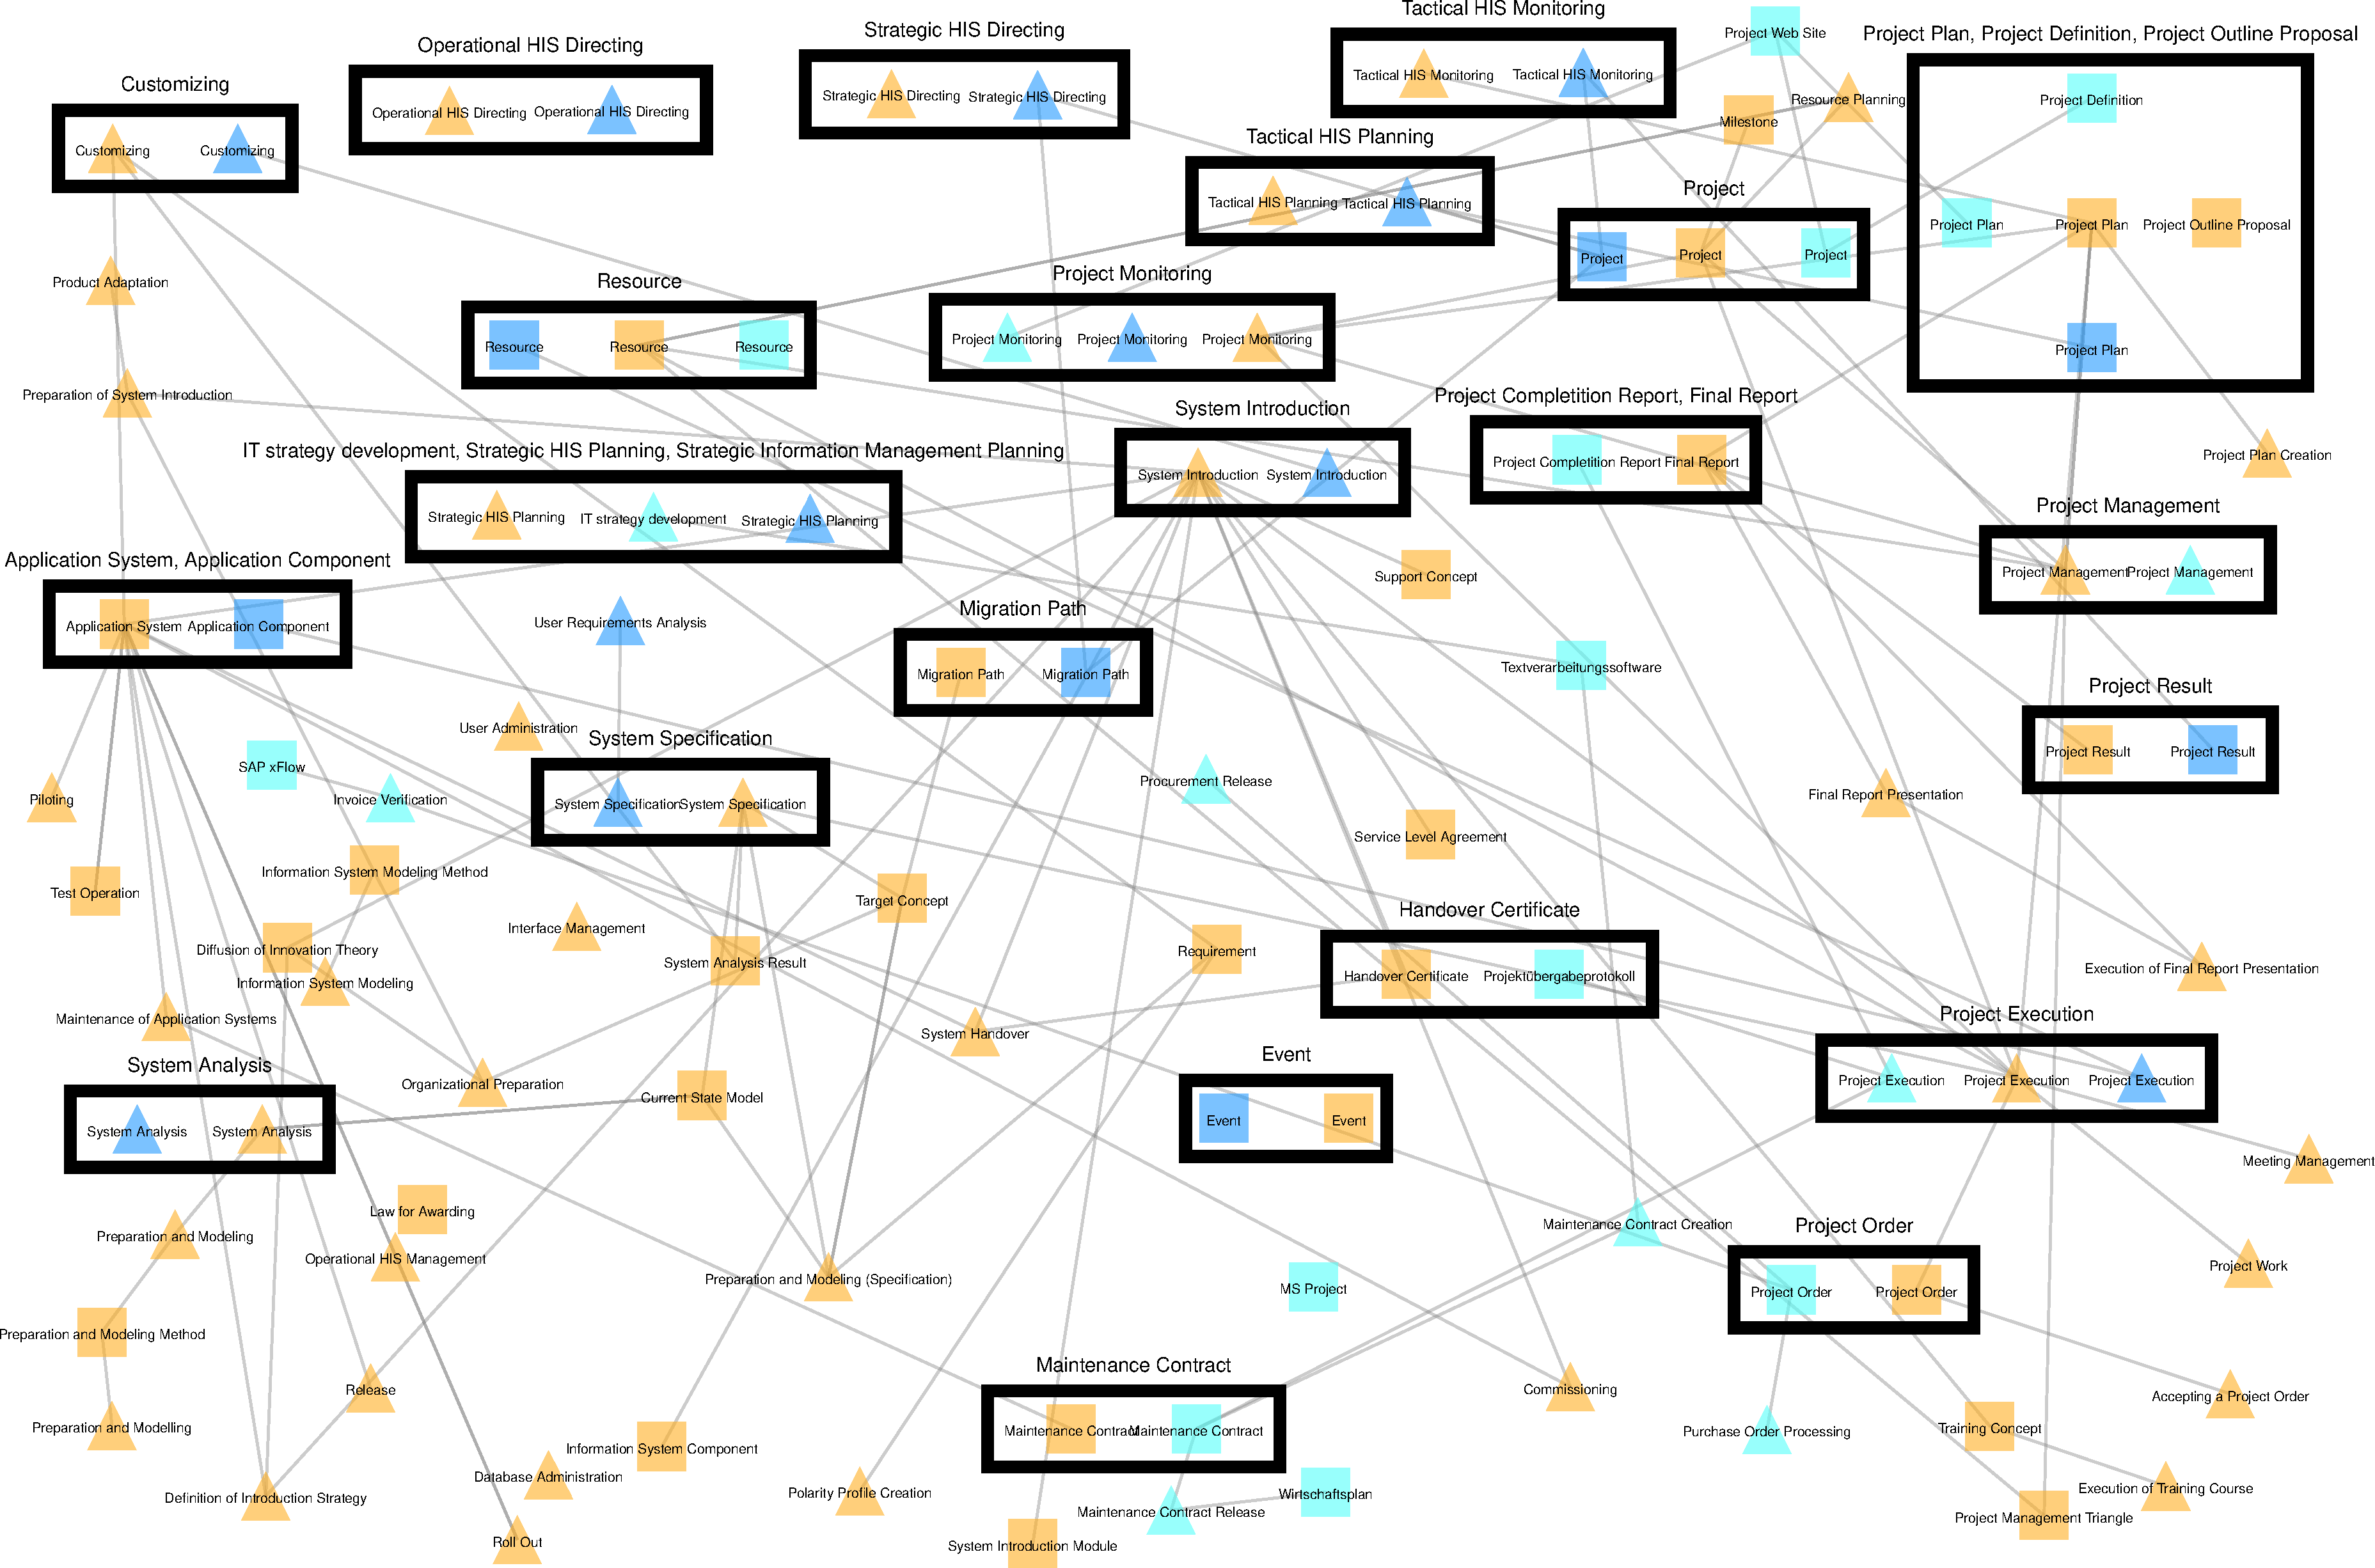
\includegraphics[width=\linewidth]{combine.pdf}
    \caption{Grouping of equivalent concepts from different sources in SNIK Graph (color coded).}% using the \enquote{combine matches} option.}
	\label{fig:combine}
\end{figure}
\vspace{-3pt}
%\noindent For citations of references, we prefer the use of square brackets and consecutive numbers, e.g. as shown by Author et al. [2], [3, pp. 5–10], as mentioned earlier [1], [3], [9]. The following bibliography provides the basic formats as a reference list with entries for journal articles [1], book chapter [2], as well as a URL [5]. For further guidance please refer to the \href{https://ieeeauthorcenter.ieee.org/wp-content/uploads/IEEE-Reference-Guide.pdf}{IEEE-Reference-Guide}.

A major difficulty in understanding the domain of HIS management is the difference in perspective and nomenclature between the different textbooks, standards and other sources.
Thus, we model each source separately and do not merge concepts pairs with the same meaning.
Those pairs are however connected by interlinks if they have a label in common and are verified manually, resulting in 713 interlinks. 
To emphasize the difference in perspective, even if the name is an exact match, the interlinks are only typed as \aurl{skos}{match} and not as the more restrictive \aurl{skos}{exactMatch} or \aurl{owl}{equivalentClass}.
\todo{Franziska or Birgit: you you have a good example from the blue book and orange book? "information managment" or something similar? Konrad: Nimm den Star um "ob/ProjectManagement".} 

[FJ] The concept "project management" both exists in a textbook (Ammenwerth) and in the knowledge about information management in a German university hospital. Grouping both concepts with the help of the star function and a a closer look at the nodes' neigborhood the user detects that the terms have a different meaning. Whereas the text book deals with the management of single projects, in the CIO's world "project management" means managing multiple projects. [FJ]
Users can group interlinked nodes together and either display them side by side or on top of each other, see \cref{fig:combine}.
As SNIK consists of more than 4000 classes, viewing large parts of it at once does not convey much information.%, see \cref{fig:much}.
To alleviate this, SNIK offers multiple exploration methods described in the following.
%\begin{figure}[h!]
%    \centering
%    \includegraphics[width=\linewidth]{much.pdf}
%    \caption{Excerpt of SNIK using the default force directed layout.}\label{fig:much}
%\end{figure}

\subsection*{Role Use}
\begin{figure}[h]
\begin{lstlisting}
SELECT DISTINCT ?inner ?middle ?outer ?outerx {
 <role> (rdfs:subClassOf|skos:closeMatch|^skos:closeMatch)* ?inner.
 ?inner meta:subTopClass meta:Role.
 OPTIONAL {
  ?inner ?p ?middle.
  ?middle meta:subTopClass meta:Function.
  OPTIONAL {
   ?middle ?q ?outer.
   ?outer meta:subTopClass meta:EntityType.
   OPTIONAL {?outer (skos:closeMatch|^skos:closeMatch|^rdfs:subClassOf)+ ?outerx.}
}}}
\end{lstlisting}
\caption{SPARQL query to generate the \emph{role use} visualization.}
\label{lst:roleuse}
\end{figure}
\vspace{-3pt}
A frequent question is, what a given role does and which information is needed for those functions represented by the entity types connected to those functions.
This question is visually answered by the \enquote{role use} feature, which arranges roles, functions and entity types in concentric circles:
(1) The first ring consists of the given role and all roles that are connected by a path of \aurl{rdfs}{subClassOf} and \aurl{skos}{closeMatch} edges.
(2) The second ring consists of all functions adjacent to roles in the inner ring.
(3) The third ring consists of all entity types adjacent to functions in the middle ring.
(4) The final ring consists of all entity types that are connected to entity types from the third ring by a path of \aurl{skos}{closeMatch} and reverse \aurl{rdfs}{subClassOf} edges.
\cref{fig:classuse}
\begin{figure}[h!]
    \centering
    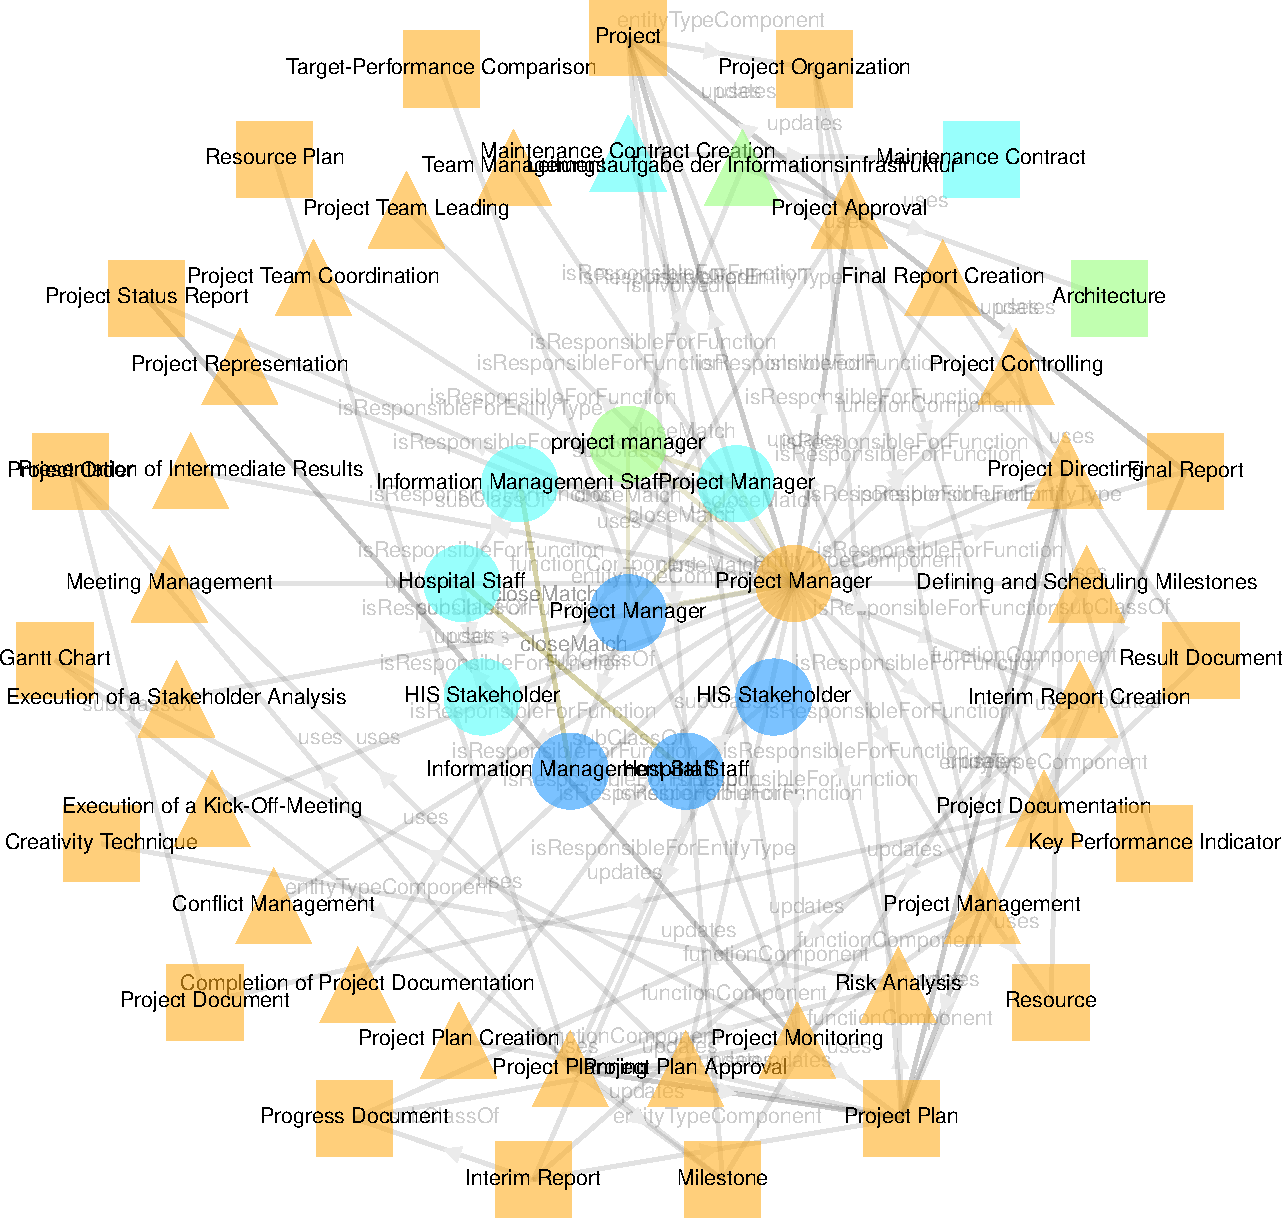
\includegraphics[width=0.6\linewidth]{class-use-project-manager.pdf}
    \caption{\emph{Role Use} of \aurl{bb}{ProjectManager}. Outermost layer ommitted due to space limitiations.}\label{fig:classuse}

\end{figure}

\section*{Approach}
At the core of SNIK Graph is incremental exploration, which starts at one or more nodes and gradually expands them to related ones.

\subsection*{Search}
\begin{figure}[h!]
    \centering
    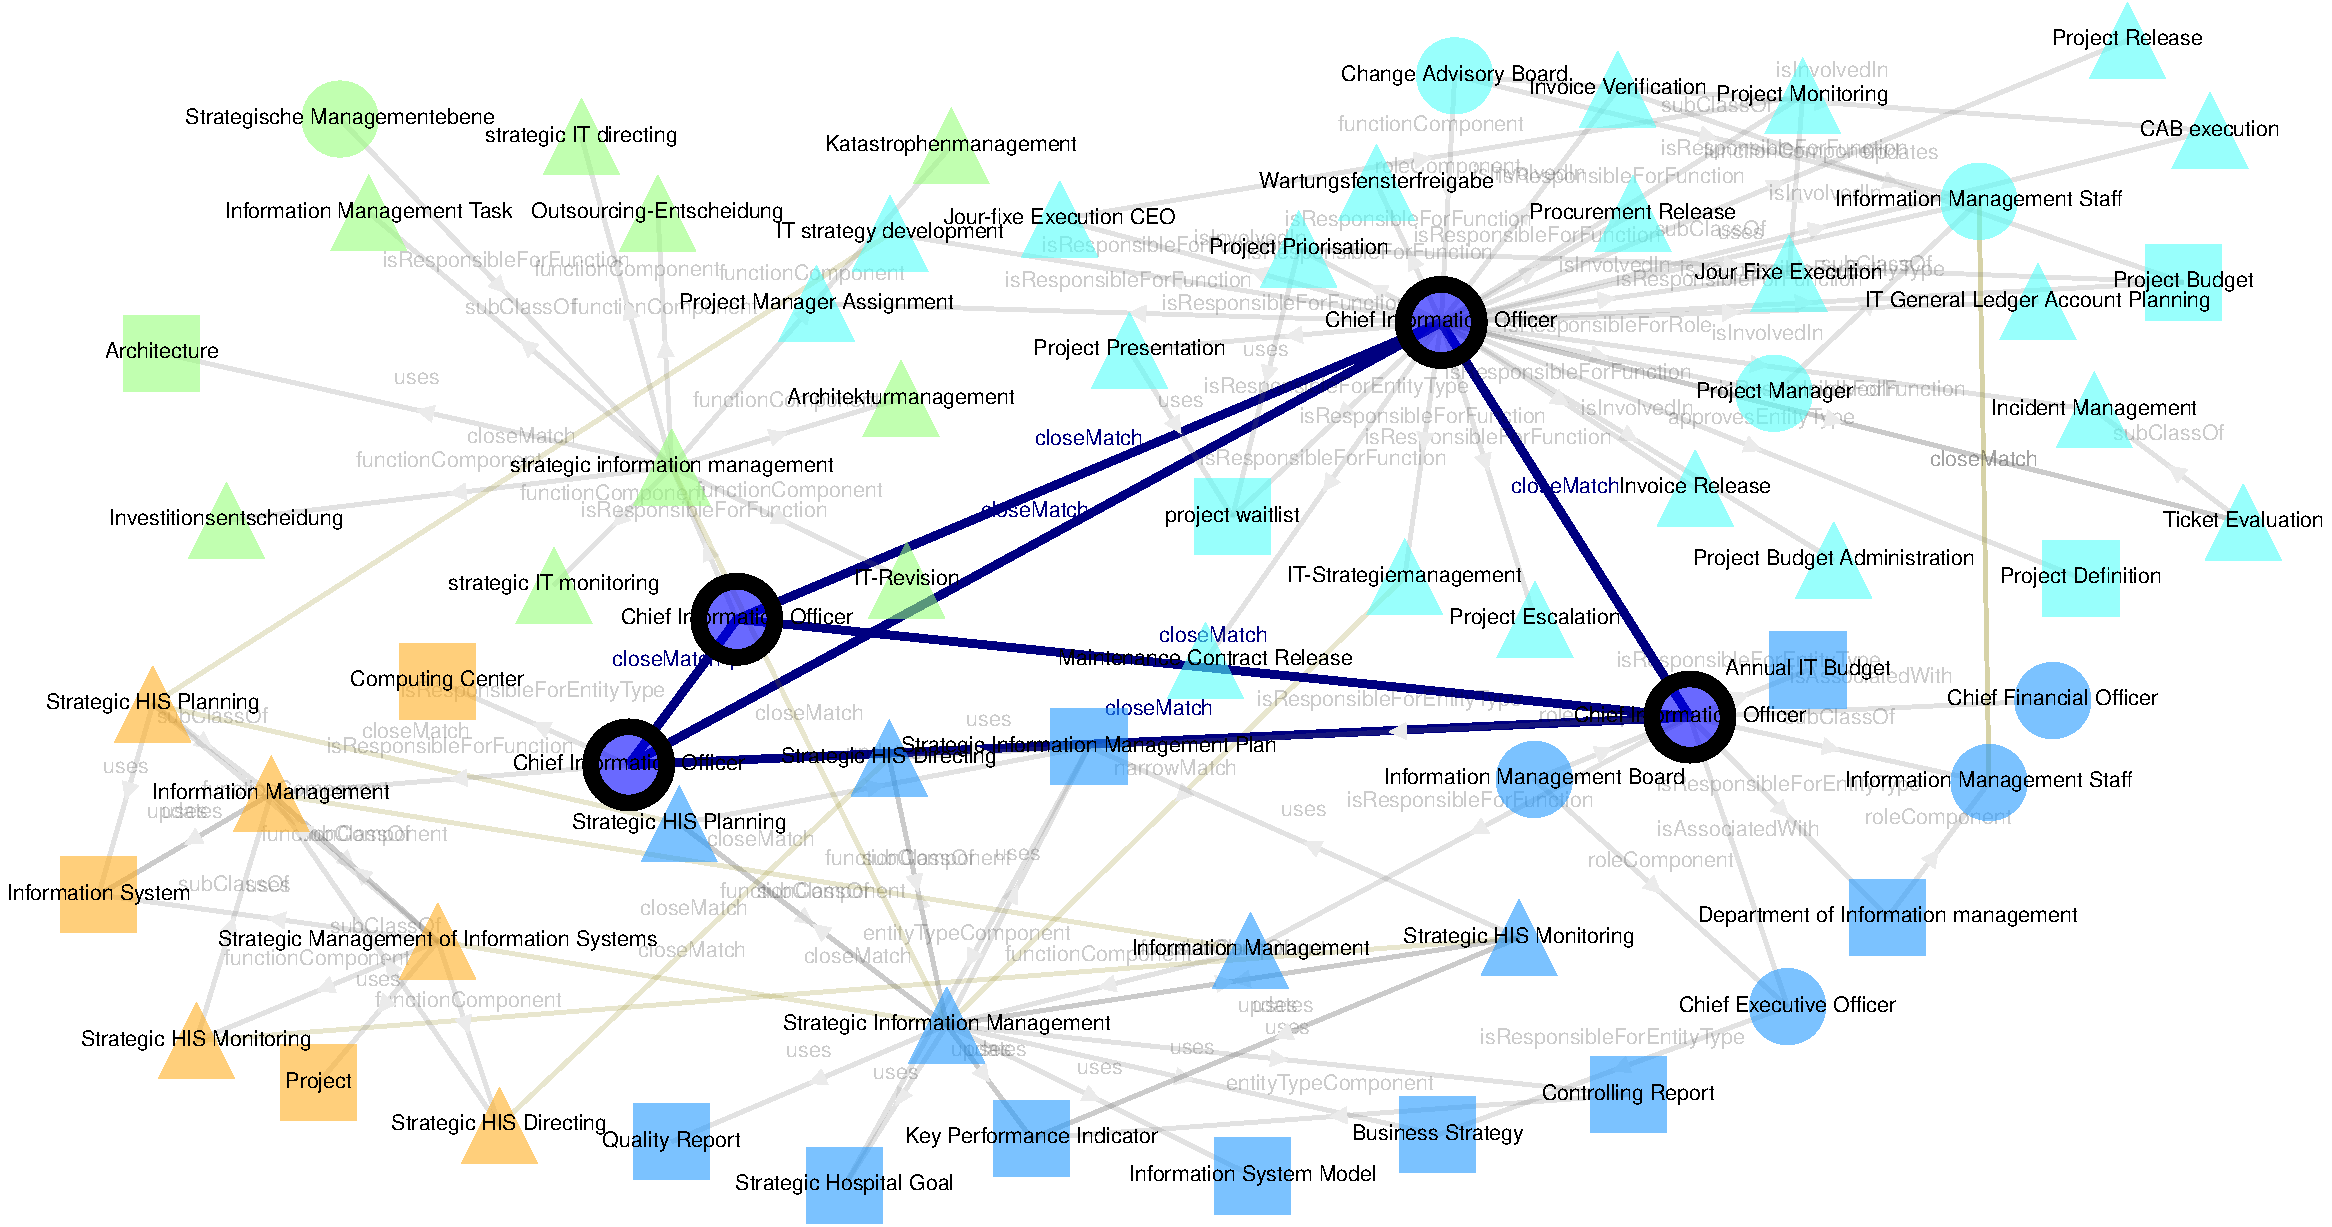
\includegraphics[width=\linewidth]{search.pdf}
    \caption{Visual search results for \enquote{Chief Information Officer} in a part of SNIK.}\label{fig:search}
\end{figure}

Due to the large amount of resources, exploration often begins with a search.
The search index is populated from the target SPARQL endpoint and is implemented using the Fuse.js library that is based on the Baeza-Yates--Gonnet algorithm~\cite{textsearching}.
Fuse.js\footnotemark{} is a light-weight, purely client side JavaScript library and presents an alternative to backend-driven indexes like Lucene.%
\footnotetext{\url{https://fusejs.io/}, \url{https://github.com/krisk/Fuse}}
This enables fast fuzzy search on any dataset loaded via SPARQL endpoint but requires waiting for index initialization on the first search of each user session.
Search results presented to the user are color coded in three categories: visible (green), invisible (yellow)%
\footnote{The resource is either \emph{filtered} or \emph{hidden}.}% \cref{sec:visibility}
 and not loaded (red)%
\footnote{The resource is included in the search index built from the SPARQL endpoint but either deleted in the graph or not loaded in the first place, such as due to configuration.}.
Each search entry of a class contains the label values of \aurl{rdfs}{label} (long form) and \aurl{skos}{altLabel} (short and alternative forms) with a weight of 0.7.
Textbook definitions are included with a weight of 0.3.
Labels of resources connected via \aurl{skos}{closeMatch} interlinks in either direction are included as well, because those resources are defined as semantically close, so we assume their labels are synonyms.
Fuzzy matching is enabled with a threshold of \num{0.25}.
The resource \aurl{bb}{ChiefInformationOfficer} can thus be found by entering either \enquote{CIO} (alternative label), \enquote{vice president} (part of the definition) or \enquote{Leiter des Rechenzentrums} (German alternative label of \aurl{ob}{ChiefInformationOfficer}).
Search results are then selected in the graph, see~\cref{fig:search}, which allows further exploration by chaining the path and neighbourhood operations described in following.

\subsection*{Shortest Paths}
\begin{figure}[h!]
    \centering
    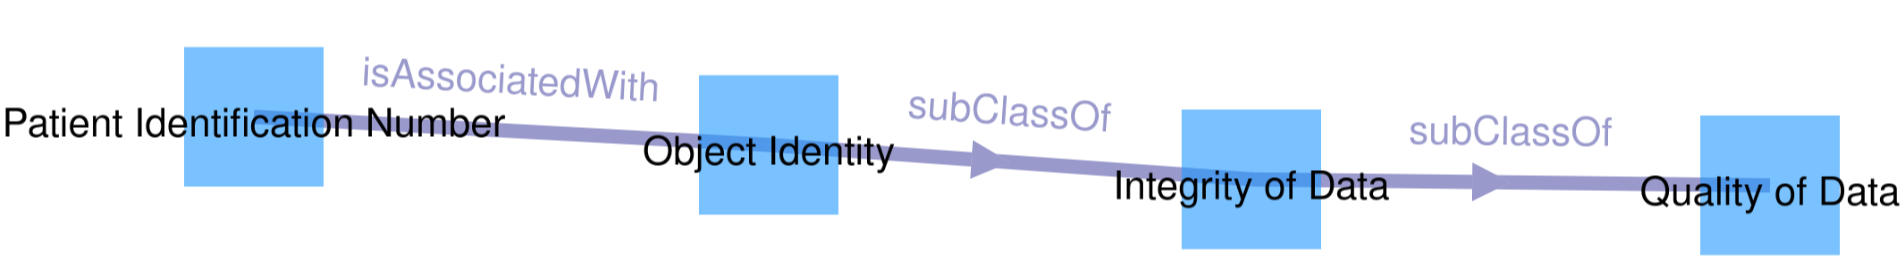
\includegraphics[width=\linewidth]{path.png}
    \caption{The shortest non-trivial path between \aurl{bb}{PatientIdentificationNumber} and \aurl{bb}{QualityOfData} in SNIK Graph.}
	\label{fig:path}
\end{figure}
\vspace{-3pt}
The shortest path is the most basic method of visualizing the relationship between two resources, see \cref{fig:path}.
We treat SNIK as an undirected graph for the calculation because the direction is often arbitrary.
Roles can be nested using \aurl{meta}{roleComponent} (\emph{has part}), which could have just as well been modelled as a \emph{part of} relation with reversed subject and object.
Another reason is that a set of resources that forms a graph connected by some symmetric property implies a complete subgraph, which negatively effects speed, memory and visibility of SNIK Graph.
For this reason, \aurl{skos}{closeMatch} and other symmetrical properties are often only sparsely modelled, and the other triples are implied.
As SPARQL endpoints, such as Virtuoso SPARQL employed by SNIK, do not perform reasoning to infer such implied triples such as those generated by symmetric properties, this would prevent the shortest path from including resources where only the opposite direction is explicitly modelled.%
\begin{figure}[h]
    \centering
    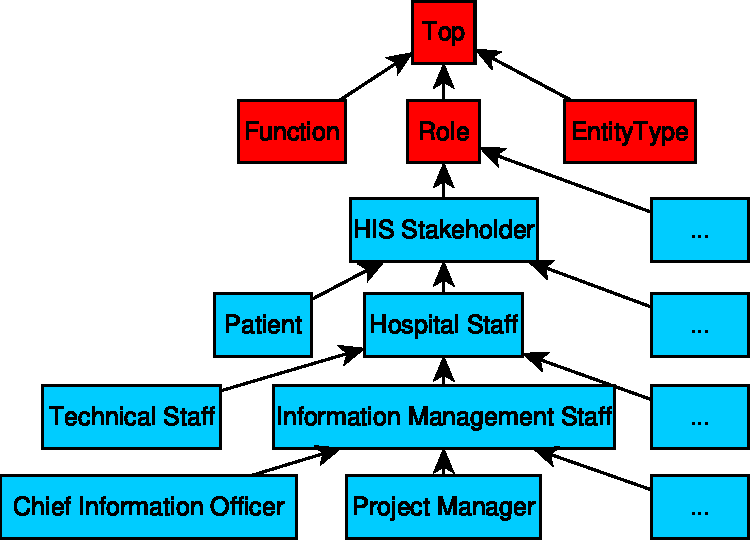
\includegraphics[width=0.5\linewidth]{hierarchy.pdf}
    \caption{Excerpt of the SNIK class hierarchy. Source: \cite{snikposter}.}
	\label{fig:hierarchy}
\end{figure}
\vspace{-3pt}
We also don't explicitly store triples inferred by transitive properties such as \aurl{rdfs}{subClassOf}, which prevents paths involving such properties from being squashed, such as the path between \emph{Project Manager} and \emph{HIS Stakeholder} in \cref{fig:hierarchy}.


%We ignore the direction of edges because, that is, which resource is the subject and the object 
The largest problem of shortest paths is however, that they are not necessarily informative to the user. 
For example, any two roles, such as \aurl{bb}{ChiefInformationOfficer} and \aurl{bb}{ChiefExecutiveOfficer}, are connected by a path of length 2 as they are all subclasses of \aurl{meta}{Role}, which the user already knows given the triangular shapes representing roles in SNIK Graph.
To exclude such trivial paths,  the meta model is not shown by default.
Furthermore, filtering, such as by knowledge source or type of relation or resource, allows further tuning of the resources that are shown and eliglible for paths.
%Further research into informative paths has been done in two bachelor theses~\cite{}.
An general approach to solve the problem of informative shortest paths is \emph{weighted shortest paths for RDF graphs (WiSP)}~\cite{wisp}.
Future work includes adopting this approach to SNIK Graph and evaluating it with its users.
Another approach is to show all short paths under a given length and let the user remove unwanted ones manually, as employed by \emph{Relfinder}~\cite{relfinder}.

\subsection*{Neighbourhood Operations}
Exploration using neighbours, that is the successive uncovering of nodes adjacent to a starting node given by a user, is a common feature of tools such as \cite{lodlive} and \cite{vizlod}.%
\subsection*{Star}
The directed and undirected star operations show nodes connected to selected nodes via all paths that contain at most one property other than \aurl{skos}{closeMatch}.
The \emph{circle star} also rearranges the nodes using the force-directed layout locally on the currently visible subgraph.
\Cref{fig:star} shows a mind map of strategic information management, created by an undirected star, which can be used by a teacher to prepare a lecture about the topic.
\begin{figure}[h!]
    \centering
    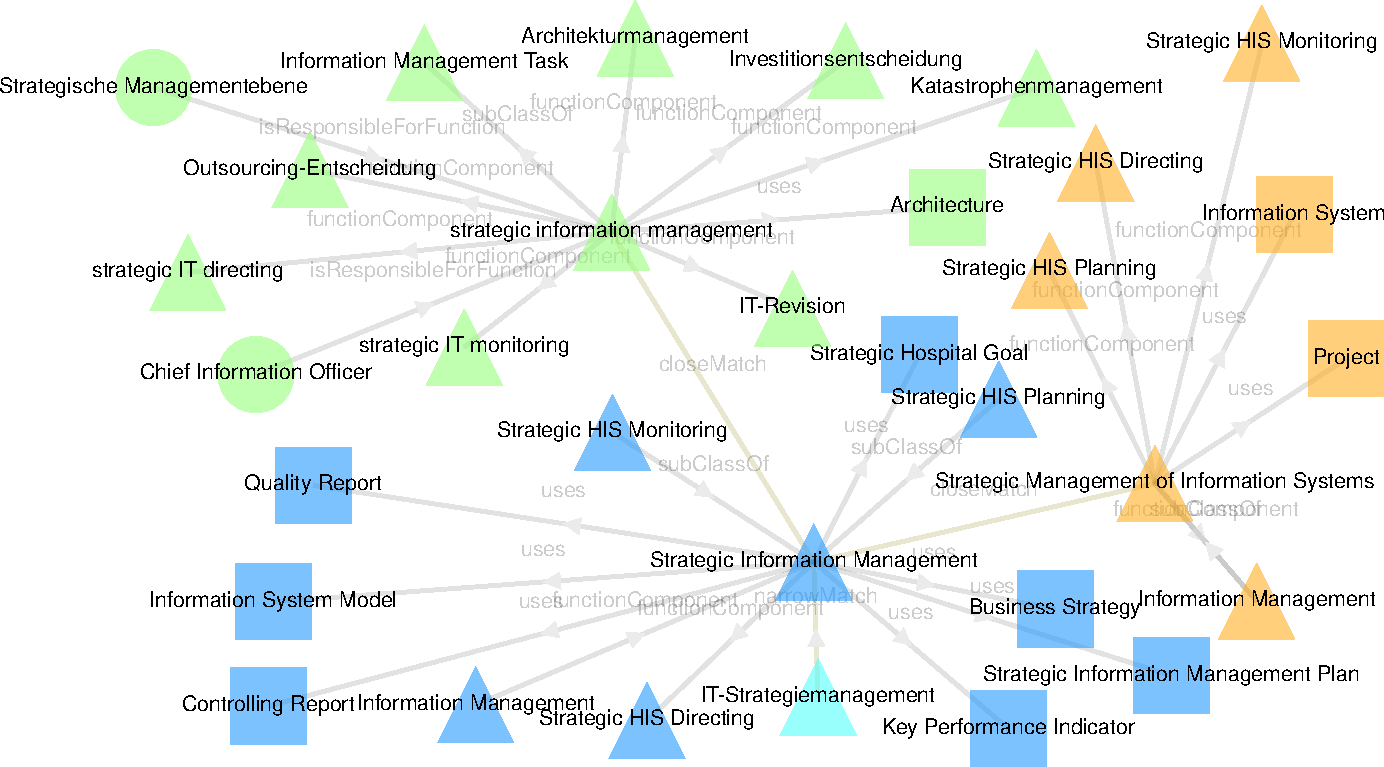
\includegraphics[width=\linewidth]{strategic-im.pdf}
    \caption{Undirected \emph{Star} of \aurl{bb}{StrategicInformationManagement}.}
	\label{fig:star}
\end{figure}
\vspace{-3pt}

\subsection*{Mixed Operations}
\subsubsection*{Spiderworm}
A \emph{spiderworm} is a path from node \emph{A} to node \emph{B} combined with a \emph{star} of \emph{B}.
\Cref{fig:spiderworm} shows how we use a spiderworm to teach a student how the new concept \enquote{quality of data} is connected the the already introduced concept \enquote{patient identification number.}

\begin{figure}[h!]
    \centering
    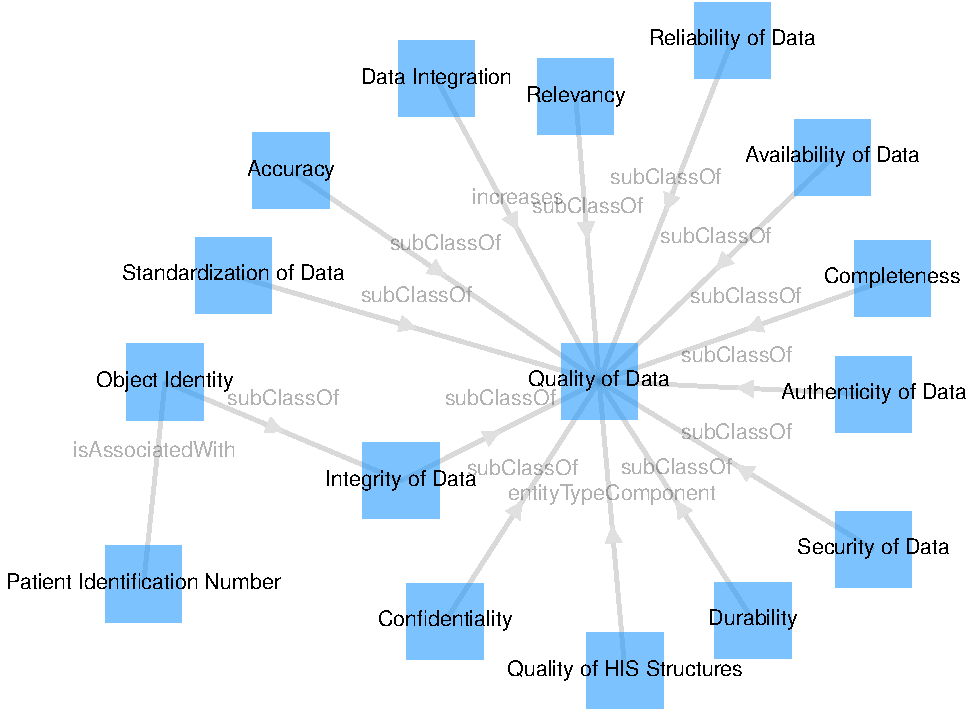
\includegraphics[width=0.5\linewidth]{spiderworm.pdf}
    \caption{\emph{Spiderworm} from \aurl{bb}{PatientIdentificationNumber} to \aurl{bb}{QualityOfData}~\cite{snikgraphposter}.}
	\label{fig:spiderworm}
\end{figure}
\vspace{-3pt}

\section*{Discussion}
% A problem is that related approaches are not available as open source ...
% this hinders analysis and slows progress, as effort is not shared and ...
\section*{Evaluation}
SNIK Graph is evaluated on the SNIK dataset, which contains textbook knowledge about the management of hospital information systems.

\section*{Discussion}
Different presentation forms are suitable for different use cases and data sets.
% RDF browsers are well suited for ...

\section*{Future Work}
\subsection*{Performance}
%On graphs of several thousand nodes, 
The performance of SNIK Graph suffers in two key areas:

%(1) Performing a force directed 
\subsubsection*{Force-Directed Layouts}
As CPUs with 6 to 16 cores become the norm, the speed penalty of single-threaded code becomes enormous.
Thus, the single-thread paradigm of JavaScript seriously hinders performance of CPU-bound applications like SNIK Graph.
While web workers\footnote{\url{https://html.spec.whatwg.org/multipage/workers.html\#workers}} offer multithreading for JavaScript applications, they posess separate memory and cause large overheads for serialization and deserialization and are thus not suited for short-lived tasks like calculating a single step of a force-directed layout for parts of a given graph.
Thus, a light-weight parallellization option is needed.
The WebAssembly \enquote{threads}-proposal\footnote{\url{https://github.com/WebAssembly/proposals/issues/14}} provides such a construct, however it is only at phase 2 \enquote{Proposed Spec Text Available}, which need to be followed by the implementation in browsers and the standardization phase.
The main developer of the Cytoscape.js library showed interest in rewriting a future version of the library in WebAssembly.

\subsubsection*{Graph Rendering}
Due to the low performance of rendering on an HTML canvas, the frame rate drops significantly below a fluent 60 frames per second.
The frame rate is especially low on large resoultions such as 4k (3840x2160) and on browsers other than Google Chrome (see table ...), where it can get as low as 2 FPS.
%Another ... incredible power of modern GPUs.

%\subsection*{Mobile Devices}

%- We also tried to automatically find the most interesting path but this was not successfull as it is subjective and the depends on the goal of the user.
%(link to AB bachelor thesis if allowed)

\begin{table}[h]
\centering
\caption{Namespaces.}
\label{tab:namespaces}
\begin{tabularx}{\linewidth}{|l|X|l|}
%\toprule
\hline
\textbf{Prefix}	&\textbf{Ontology}				&\textbf{Source}\\
%\midrule
meta	&\url{http://www.snik.eu/ontology/meta}		&Meta Model\\ \hline
bb		&\url{http://www.snik.eu/ontology/bb}		&Textbook~\cite{bb}\\\hline
ob		&\url{http://www.snik.eu/ontology/ob}		&Textbook~\cite{ob}\\\hline
%\url{http://www.snik.eu/ontology/he}		&Textbook~\cite{he}\\\hline
%\url{http://www.snik.eu/ontology/ciox}		&CIO Interview\\\hline
%\url{http://www.snik.eu/ontology/it4it}		&Standard~\cite{it4it}\\\hline
%k\bottomrule
\end{tabularx}
\end{table}

\noindent Tables and Figures should be centered.

\begin{enumerate}[align=left, labelwidth=1ex]
    \item Numbering may be used, too.
    \item ...
\end{enumerate}

\noindent Equations should be centered and set on a separate line.
\begin{equation}
    x+y=z
\end{equation}


\section*{Acknowledgement}
This work is supported by the DFG (German Research Foundation) under the Project SNIK, Grant no. 1605/7-1 and 1387/8-1. SNIK Graph is presented in poster form at \cite{snikgraphposter}.
\section*{References}

%\printbibliography[heading=none] %Uncomment if using biblatex. This command generates the refrences section automatically.
\bibliographystyle{plain}
\bibliography{paper,snik,relatedwork}

\end{document}
